\chapter{Preliminaries}

\section{Cellular Automata}

A cellular automaton (CA) is a computational model that performs multiple parallel computations, each depending only on local interactions, to produce complex global behaviour. We define a CA formally as follows.

\begin{definition}[Cellular Automaton]
A cellular automaton is an $n$-dimensional finite grid of computational units called cells. Each cell $c_i$ is characterised by:
\begin{itemize}
  \item A discrete state variable $\sigma_i(t) \in \Sigma$, where $i$ indicates the index of the cell in the lattice, $t$ indicates the current time step, and $\Sigma$ denotes the finite set of all state variables.
  \item A finite local neighbourhood set $\mathcal{N}(c_i)$ with cardinality $N$.
  \item A transition function $\phi:\Sigma^N \to \Sigma$ which takes local neighbour states as input. This is also known as the CA "rule".
\end{itemize}

At each time step, the state of each cell is simultaneously updated according to the transition function. That is, $\sigma_i(t+1) = \phi( \:\{ \sigma_j(t) \: | \: c_j \in \mathcal{N}(c_i) \} \:)$

\end{definition}
Due to the breadth of systems studied in CA literature, the constraints of this definition are often altered to produce interesting arrangements. For example:
\begin{itemize}
  \item The structure need not be a square grid. CA have been studied on hexagonal grids[CITE], aperiodic tilings such as as the Penrose pattern[CITE], or even randomly generated partitions like the Voronoi tessellation[CITE].
  \item The system need not be deterministic. Probabalistic cellular automata (PCA)[CITE] have stochastic transition functions which describe a probability distribution of possible outcomes for any given input. PCA are able to model random dynamical systems in the real world from stock markets[CITE] to infectious diseases[CITE].
  \item The state space $\Sigma$ need not be finite. In this thesis we will explore multiple possible state variable representations including bit arrays and continuous vectors.
\end{itemize}
For the purpose of this thesis, we will assume the original definition of CA unless otherwise stated. 

\subsection{Neighbourhood Functions}
We consider a "neighbourhood function" for each cell $c_i \mapsto \mathcal{N}(c_i)$. This makes it easier to discuss neighbourhood sets of cells in the CA, each of which are typically homogenous.\\

On any particular CA geometry, there are many possible neighbourhood functions. When defining the neighbourhood function, we select a distance metric $d:\mathbb{R}^n \times \mathbb{R}^n \to \mathbb{R}$ to measure the proximity of two cells and we set a threshold $T$ under which we consider the two cells to be within each other's neighbourhood.
\[c_i \in \mathcal{N}(c_j) \iff d(c_i, c_j) \leq T\]

There are two neighbourhoods that are frequently used on Euclidean lattices. The \textit{von Neumann neighbourhood} contains all cells within a Manhattan distance of 1. For a 2D square lattice, this contains the cell itself and the 4 cells in the cardinal directions. For a 3D cubic lattice, it contains the central cell and a 6-cell octahedron around it. The \textit{Moore neighbourhood} contains all cells at a Chebyshev distance of 1. For a 2D square lattice, this is the central cell with the 8 neighbouring cells in a square around it. In the 3D case, it is a cube.

\begin{figure}[!h]
\centering
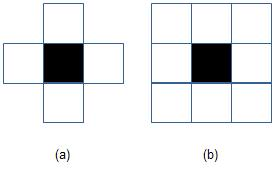
\includegraphics[width=0.4\textwidth]{images/neighbourhoods.png}
\caption{(a) von Neumann Neighbourhood and (b) Moore neighbourhood on a 2D square lattice \cite{debasis2011survey}}
\label{fig:neighbourhoods}
\end{figure}

In a finite grid CA, border cells must be given special consideration since they do not have the same number of neighbours as interior cells and therefore cannot share the same neighbourhood function. One option is to define a case-wise neighbourhood function with different behaviour for border cells. Another option is to freeze the state of border cells. In the field of partial differential equations, this is known as setting "fixed boundary conditions".  The problem can also be circumvented entirely by relaxing the finite grid assumption and allowing cells to "wrap around" the grid. This is known as setting "periodic boundary conditions" and can be imagined visually as running the CA on an infinite periodic tiling or, alternatively, on a torus.\\


\subsection{Conway's Game of Life}
The most popular example of a CA is the Game of Life (henceforth "Life") formulated by John Conway in 1970 \cite{gardner1970fantastic}. It consists of a 2D grid of cells, each with a boolean state variable signifying that the cell is either "alive" or "dead". The transition rule is a function of the cell's own state $S_i(t)$ and the number of living individuals in the cell's Moore neighbourhood (excluding itself), denoted $n$. This is as follows:

\begin{equation}
  \phi(S_i(t), n) = 
\begin{cases}
  0 & S_i(t) = 1 \text{ and } n < 2 \text{  (Death by "loneliness")}\\
  0 & S_i(t) = 1 \text{ and } n > 3 \text{  (Death by "overcrowding")}\\
  1 & S_i(t) = 1 \text{ and } n \in \{2,3\} \text{  (Survival)}\\
  1 & S_i(t) = 0 \text{ and } n = 3 \text{  (Resurrection)}\\
  0 & \text{otherwise}
\end{cases}
\end{equation}

Despite its simplicity, Life is Turing complete. There has been a lot of experimentation with Life to discover and classify patterns that can exist within it. Some examples include periodic oscillators like the \textit{beacon} which has period 2 or still lifes like the \textit{block} which are fixed-point solutions \ref{fig:life-patterns}. These can be thought of as having period 1. There are also periodic patterns that move across the lattice such as the \textit{glider} pattern.

\begin{figure}[!h]
\centering
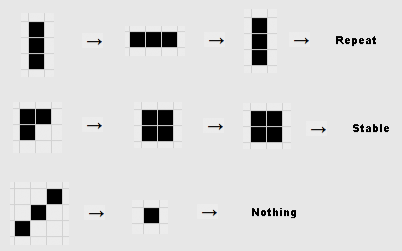
\includegraphics[width=0.8\textwidth]{images/life-patterns.png}
\caption{Patterns within the Game of Life. From top to bottom: blinker, block, unnamed \cite{lipa}}
\label{fig:life-patterns}
\end{figure}


\begin{figure}[!h]
\centering
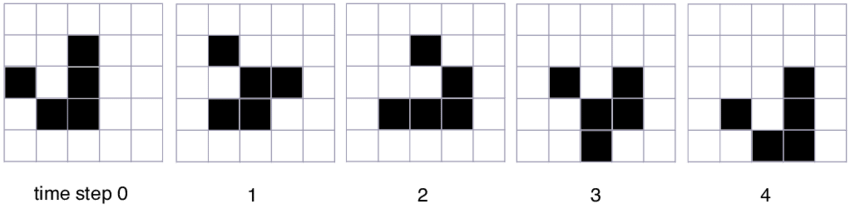
\includegraphics[width=0.8\textwidth]{images/life-glider.png}
\caption{The glider pattern within the Game of Life \cite{dorin2012framework}}
\label{fig:life-glider}
\end{figure}

\subsection{Wolfram's Classification}

The choices of lattice geometry, neighbourhood function, state variable, and transition rule define the behaviour of a CA. Fixing the former three factors, Wolfram \cite{wolfram1986theory} has classified CAs based on transition rules as follows:
\begin{enumerate}
  \item Class 1 (Null) : Rules that lead to a trivial, uniform state
  \item Class 2 (fixed-point + periodic) : Rules that lead to stable or periodic patterns
  \item Class 3 (Chaotic) : Rules that lead to chaotic patterns
  \item Class 4 (Complex) : Rules that lead to complex, long-lived impermanent patterns
\end{enumerate}

\textbf{Elementary cellular automata} are defined on the simplest nontrivial lattice, a finite one-dimensional chain. The neighbourhood of each cell contains the cell itself and the two cells adjacent to it on either side. The state variable is a boolean which means there are $2^3 = 8$ possible neighbourhood state configurations. A transition rule maps each of these neighbourhood states to a resultant state and can therefore be represented as an 8-digit binary rule table $(t_7t_6t_5t_4t_3t_2t_1t_0)$ where configuration $(000)$ maps to $t_0$, $(001)$ maps to $t_1$, ..., and $(111)$ maps to $(t_7)$. Consequently there are $2^8=256$ possible transition functions for elementary CA. Figure \ref{fig:rule-space} illustrates the distribution of classes in this rule space as we vary $p$, the proportion of 1s in the rule table. \\

The Wolfram code, a number between 0 and 255 obtained by converting the binary rule table to decimal, is the standard naming convention for these rules. Rule 110 is particularly notable as it can exhibit class 4 behaviour \cite{wolfram2002} and has been proven to be Turing Complete \cite{cook2004universality}. Figure \ref{fig:rule-110} shows an example progression of a Rule 110 system. Each row of pixels represents the state of the automaton at one snapshot in time with the topmost row representing the randomized initial state. It shows the emergence, interaction, and subsequent dissipation of multiple long-lived impermanent patterns.

\begin{figure}[!h]
\centering
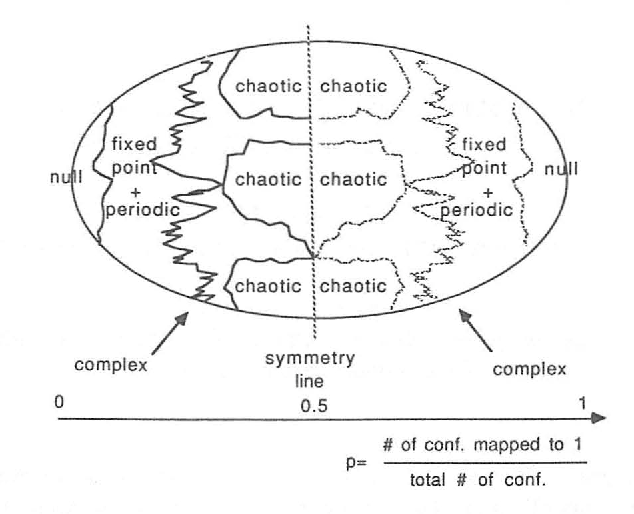
\includegraphics[width=0.9\textwidth]{images/rule-space.png}
\caption{Schematic illustration of elementary CA rule space from Li and Packard \cite{li1990structure}}
\label{fig:rule-space}
\end{figure}

\begin{figure}[!h]
\centering
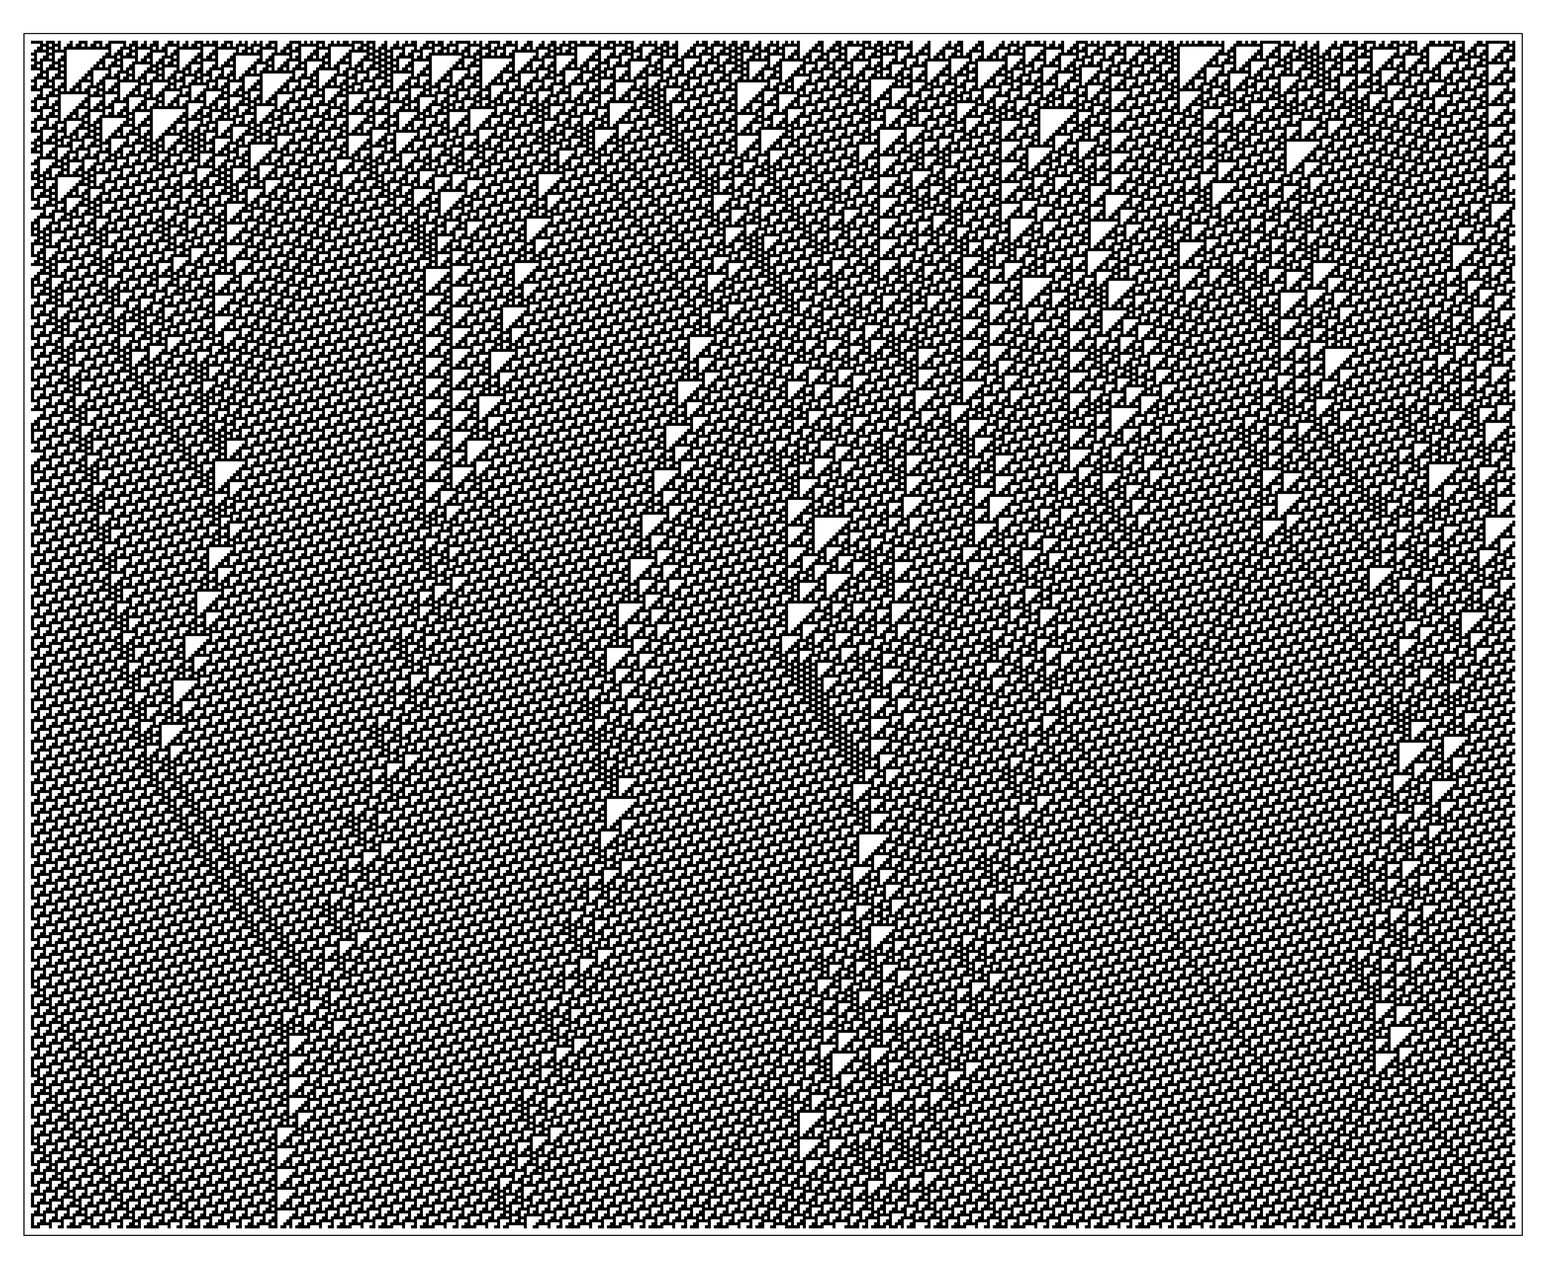
\includegraphics[width=0.9\textwidth]{images/rule-110.png}
\caption{Rule 110 progression with random initialisation \cite{wolfram2002}}
\label{fig:rule-110}
\end{figure}

\section{Morphogenesis}
Morphogenesis is the process by which a system develops into a particular shape or pattern. 
Biologically, this is seen in most multicellular organisms which can robustly develop specialised organs and intricate skin patterns without any centralised decision-making.
Through simple rules encoded in the genome and homeostatic feedback loops enforced through chemical signalling, a tissue knows exactly how to grow and when to stop.\\

Emulating this behaviour \textit{in silico} can provide great insight into the way self-organising and self-repairing biological systems function.
Cellular automata are a promising model of computation for artificial life simulation because, much like biological agents, their behaviour follows logically from combining information in their surroundings and internal programming.
In the context of morphogenesis, we are interested in rules that form stable class 2 patterns from random initial conditions.
We are also interested in rules that are resistant to noise.
This is analogous to the behaviour of biological cells which grow into stable configurations and are robust to perturbation and damage during growth.